% !TEX root = ../main.tex

\section{The Core Library}
\label{sec:rust:core}

As described in \autoref{sec:rcl}, the \gls{rcl} defines the \emph{core} functionality of the {\rust} language.
The \gls{rcl} does not have any library dependencies, but in order to use the library without \gls{rsl}, a few definitions are needed.
These definitions are given in \autoref{tab:core:definitions}.

\begin{table}[H]
  \centering
  \begin{tabular}{l | l}
    \textbf{Functions} & \textbf{Description} \\
    \hline
    \code{memcpy, memcmp, memset} & Basic memory management \\
    \code{rust\_begin\_unwind}    & Handles panicking \\
    \hline
  \end{tabular}
  \caption{External dependencies of \gls{rcl}}
  \label{tab:core:definitions}
\end{table}

The memory management functions given in \autoref{tab:core:definitions} are provided by \lib{newlib} and are exposed through the \lib{startup} library described in \autoref{sec:startup}.
These functions provide the basic memory management that is needed in order to utilize the parts of \gls{rsl} that defines dynamically allocated data structures.

\concept{Panicking} is {\rust}'s way of unwinding the currently executing thread, ultimately resulting in the thread being terminated.
A panic in {\rust} can happen, e.g. when an array is indexed out of bounds, which causes the \code{rust\_begin\_unwind} function to be called.
The \code{rust\_begin\_unwind} is also defined in \lib{startup}, but the implementation is only an infinite loop to aid debugging.
In contrast, the definition of \code{rust\_begin\_unwind} given in \gls{rsl} will abort the program and print an error message.

\section{The Allocation Library}
\label{sec:rust:allocation}

Heap allocation is introduced in a library called \lib{alloc}.
The library defines the managed pointer, \code{Box}, which is {\rust}'s main means of allocating memory on the heap.
Also, the allocation library defines the types \code{Rc} and \code{Arc}, which are {\rust}'s \emph{reference counted} and \emph{atomically reference counted} heap pointers.

\begin{listing}[H]
  \begin{rustcode}
fn rust_allocate(usize, usize) -> *mut u8;
fn rust_deallocate(*mut u8, usize, usize);
fn rust_reallocate(*mut u8, usize, usize, usize) -> *mut u8;
  \end{rustcode}
  \caption{External dependencies of the \lib{alloc} library}
  \label{tab:alloc:external-funcs}
\end{listing}

The allocation library is by default dependent on \lib{libc}, but this dependency can be broken by supplying the \flag{--cfg feature="external\_funcs"} flag to the compilation process.
When breaking this dependency, the allocation library requires the functions in \autoref{tab:alloc:external-funcs} to be defined elsewhere.
Note that these functions map directly to the \code{alloc}, \code{dealloc}, and \code{realloc} functions, which all are part of {\newlib}.
This design makes it easy to include the {\lib{alloc}} library for new platforms like {\rg}.

\section{The Collection Library}

The {\rust} \lib{collections} library provides general purpose data structures.
Out of these data structures the \code{Vector} (a growable heap allocated list) and the \code{String} (heap-allocated mutable strings) are the most notable.

As one would expect, the \lib{collections} library depends on the \lib{alloc} library, as it needs to allocate memory on the heap.
\texttt{collections} also depends on the \texttt{unicode} library because all strings in {\rust} are UTF-8 encoded.

\section{The Rust Embedded Library}
\label{sec:rel}

The libraries mentioned in the previous sections provides core language constructs and dynamic heap allocation.
Together they form a strong foundation for new {\rust} programs, without depending on an \gls{os}.
We have composed these libraries into what we refer to as the \gls{rel}, and the dependencies of these libraries are is shown \autoref{fig:rust:rel}.

\begin{figure}[H]
  \begin{center}
    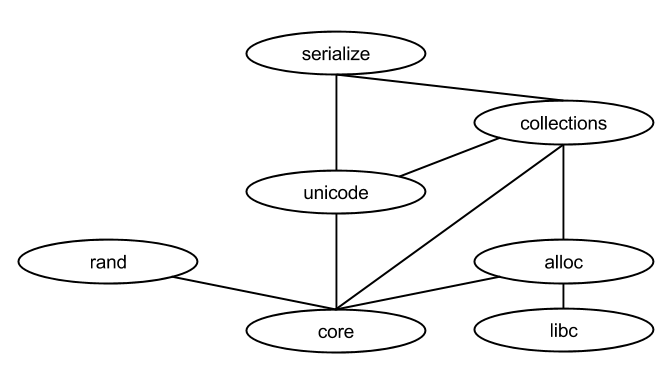
\includegraphics[scale=0.3]{figures/background/rust/embedded-rust-lib.png}
  \end{center}
  \caption{Rust Embedded Library}
  \label{fig:rust:rel}
\end{figure}

It is important to note that \gls{rel} is just a way to provide a well-defined definition of the {\rust} language for an embedded system.
\gls{rel} is, unlike \gls{rsl}, not built as a facade, it is nothing but a collection of freestanding {\rust} libraries that are suited for an embedded system.
However, the libraries that make up \gls{rel} needs to be conditionally compiled for the Cortex-M3 architecture, and this is described in \autoref{chap:build}.
